\chapter{Recreational Mathematics}
\label{chap:recreationalMathematics}
\myTop{It is important to understand what recreational mathematics is in order to get a better understanding of the \rubik{}. The \rubik{} is related to other recreational mathematical puzzles, which have inspired the \rubik{} and are simpler to understand at first grasp, than the \rubik{}. This chapter presents a definition of recreational mathematics and a few examples of recreational mathematical puzzles other than the \rubik{}.}
\section{Definition}
Recreation means to do something which is amusing or relaxing. Mathematics is somewhat harder to give a precise definition of, due to the vast amount of subjects that fall under this term. Most people do however have a common idea of what mathematics is.

Recreational mathematics is hereby defined as mathematical problems, puzzles or games which are fun and interesting to laymen. \cite{Singmaster98} \cite[18]{Trigg78}
\section{Puzzles}
This project is dedicated to the \rubik{} and the cube will be covered in detail later in this report. This section will instead describe some puzzles related to the Rubik's cube.

	\subsection{Magic Square}
\label{sec:magicSquare}
A \msquare{} is a square which is divided into a number of subsquares. The number of subsquares on any side is refered to as the ``order'' of that \msquare{}. In each subsquare there is a positive integer. In order for the \msquare{}, to be ``magical'', the sum of any row, column or diagonal must be the same, this sum is refered to as the magic constant.

The \msquare{}\cite{aiden06} originantes from ancient China. It was said that the people near the river Lo made offerings. Every time they made an offering a tortoise emerged from the river. On the back of the tortoise there was said to be a \msquare{}.

The \msquare{} from this tale was a 3 order \msquare{}. This is not the only order in which a \msquare{} can be created; it is possible to make an ``$n$'' order \msquare{}. Although it has been proven that it is not possible to make a second order \msquare{}.

In order to solve the \msquare{}, it is needed to know the magic constant -- the constant which every row, line and diagonal adds up to for the given order $n$. This constant can be computed with the formula in \ref{align:magicConstant}.

\begin{align}
\label{align:magicConstant}
	M(n) = \frac{n \cdot (n^2+1)}{2}
\end{align}

The proof of this formula is quite straight forward. As the table \ref{tab:magicSquareOrder3} illustrates, a \msquare{} of the order 3 contains the numbers from 1 to 9. Generally a \msquare{} of the order $n$ contains the numbers from 1 to $n^2$.

The sum of the numbers of a row in a \msquare{} is equal to the magic constant. If the magic constant is multiplied by the order $n$ it would be equal to the sum of alle the integers, since each number only occurs once in a \msquare{}.

\renewcommand{\arraystretch}{1.3}
\begin{table}[h]
	\centering
		\begin{tabular}{|c|c|c |@{\vrules}| c|}
			\hline
			6&1&8&15 \\
			\hline
			7&5&3&15 \\
			\hline
			2&9&4&15 \\
			\noalign{\hrules}
			15&15&15&45 \\
			\hline
		\end{tabular}
	\caption{\myCaption{A \msquare{} of the order 3, by adding the three numbers in any row, column or diagonal, the magic constant is seen to be 15}}
	\label{tab:magicSquareOrder3}
\end{table}

The equation \ref{proof:magicConstant1} can be rewritten into the equation \ref{proof:magicConstant2}(See proof of the right hand side transcription in appendix X).

\begin{align}
\label{proof:magicConstant1}
	n \cdot M \left( n \right) = \sum ^{n^2}_{i = 1} i = 1 + \cdots + n^2
\end{align}
\begin{align}
\label{proof:magicConstant2}
	n \cdot M \left( n \right) = \frac{n^2 \cdot \left( n^2 + 1 \right)}{2} \\
\label{proof:magicConstant3}
	M \left( n \right) = \frac{n \cdot \left( n^2 + 1 \right)}{2} 
\end{align}

The equation \ref{proof:magicConstant3} shows the function which gives the magic constant for a \msquare{} of the order $n$.

Variations of the \msquare{} exists. For example the numbers which can be inserted into the subsquares, could exeed $n^2$. This would change the magic constant. A \msquare with the intergers 1 to $n^2$ within its subsquares is called a ``Normal \msquare''. %input/introduction/recreationalMathematics/magicSquare %Denne sti skal bruges n�r rapporten samles!
	\subsection{Magic Cube}
\label{sub:mcube}



%\begin{figure}[h]	\centering		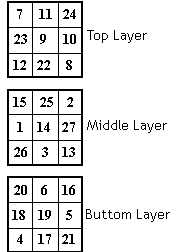
\includegraphics[scale=0.8]{input/pics/presentMagicCube2}	\caption{\myCaption{This is a magic cube split up into 3 magic squares.}}	\end{figure}



\begin{figure}[b]
	\centering
		\subfloat[\myCaption{Top layer.}]{
		
		\begin{tabular}{|c|c|c|}
			\hline
			7&11&24 \\ \hline
			23&9&10 \\ \hline
			12&22&8 \\ \hline
		\end{tabular}
		}
		\hspace{0.02\textwidth}
		\subfloat[\myCaption{Middle layer.}]{
		\begin{tabular}{|c|c|c|}
			\hline
			15&25&2 \\ \hline
			1&14&27 \\ \hline
			26&3&13 \\ \hline
		\end{tabular}

		}
		\hspace{0.02\textwidth}
		\subfloat[\myCaption{Buttom layer.}]{ 
		\begin{tabular}{|c|c|c|}
			\hline
			20&6&16 \\ \hline
			18&19&5 \\ \hline
			4&17&21 \\ \hline
		\end{tabular}
		}
		\caption{\myCaption{This is a magic cube split up into 3 magic squares.}}
		\label{fig:presentMagicCube}
\end{figure}



Both a \msquare{} and a \mcube{} have a magic constant, which can be the sum of each row, column and pillar. See figure \ref{fig:presentMagicCube}.
 However this is where the similarity ends. There are also similarities between the \mcube{} and the \rubik{} which will be elaborated on later. 

We have shown how to calculate the magic constant in a \msquare{}.
In a  \mcube{} there is not a big difference in the formula to calculate the magic constant.
\begin{equation}
	M(n)=\frac{n \cdot (n^3+1)}{2}
\end{equation}
As shown in the formula the only difference is the power of $n$ that is changed from 2 to 3.
See appendix \ref{sec:proofOfMagicConstant} for an explanation.

To create a  \mcube{}, there are some parts that need to be explained.
All these basics are shown on figure \ref{fig:cubeparts}.

\begin{figure}[htb]
	\centering
		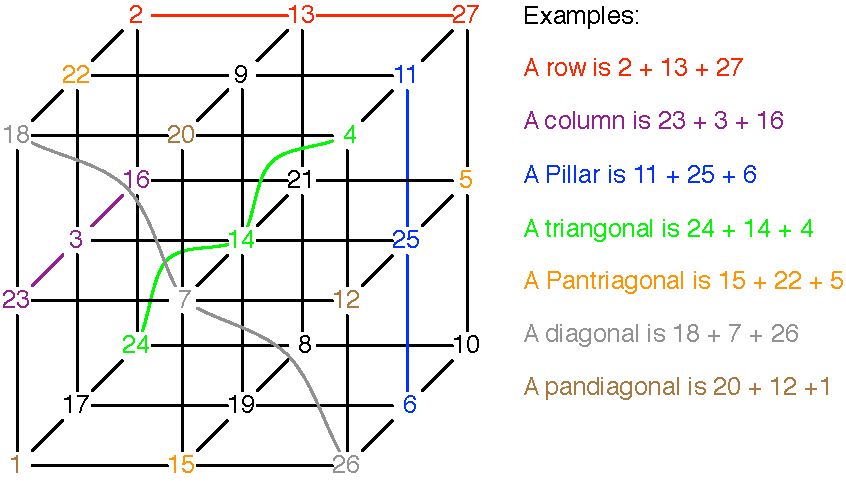
\includegraphics[scale=0.5]{input/pics/cubeparts.pdf}
	\caption{\myCaption{This is a Magic Cube where the colors show all of the parts.}}
	\label{fig:cubeparts}
\end{figure}

Because of all these different parts there are a lot of different ways to define  \mcube{}s.
The simplest of them all is a simple  \mcube{}. The only requirements to make such a cube is the following:
\begin{itemize}
	\item All 9 rows, columns and pillars must be equal to the magic constant.
	\item All 4 triagonals must also equal the magic constant.
\end{itemize}

\begin{figure}[htb]
	\centering
		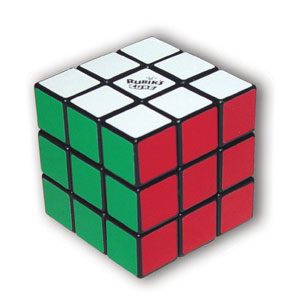
\includegraphics[scale=0.4]{input/pics/rubiksCube}
	\caption{\myCaption{This is a Rubik's Cube.}}
	\label{fig:rubiksCube}
\end{figure}

When looking at the \rubik{} it is easy to see that it looks a lot like the \mcube{}. 
There are two differences. 
The first is that the \mcube{} consists of numbers whereas the \rubik{} has colors, which are different on each \face{}.
The other difference is that the \mcube{} has a number in the center where the \rubik{} center is invisible and out of importancy. This \mcube{} should not be confused with the later presented \mcube{} made by \erno{}.
 %input/introduction/recreationalMathematics/magicCube %Denne sti skal bruges n�r rapporten samles!
	\subsection{Magic Puzzle}
The \mpuzzle{} is also known as the 15-puzzle \cite[pp. 48-50]{Larsen81}. It is a puzzle that consists of a tray with 15 square tiles and an empty square arranged in a 4x4 contraption.

It has never been discovered who actually invented the \mpuzzle{}, but Samuel Loyd who was an American chess player and puzzle author claimed that he invented the \mpuzzle{} and therefore he got the credit. This is turned down by a research of Jerry Slocum. He discovered that there was a wooden version of the game already in 1865, this was manufactured by the Embossing Co. Jerry Slocum searched for the patent and found it, US 50.608 and was applied by a Henry May. 

Jerry Slocum also found a patent by Ernest U. Kinsey that was published August 20th 1878. This version by Ernest U. Kinsey was a 6x6 version of the puzzle which also prevented the tiles from being lifted out.

\subsubsection {Permutations}
The tiles in a \mpuzzle{} can be arranged in $16!$ different positions \cite{jaapsch}. This limit can not be reached because you have to make a permutation to switch the tiles. The permutation must be an even or odd number of transpositions depending on where the position of the empty square is.

The tiles are often numbered or labeled with small pictures which when assembled correctly form a larger picture.

\begin{figure}[htb!]%
	\center
	\subfloat[\myCaption{Figure of Magic Puzzle.}]{\label{fig:MagicPuzzle}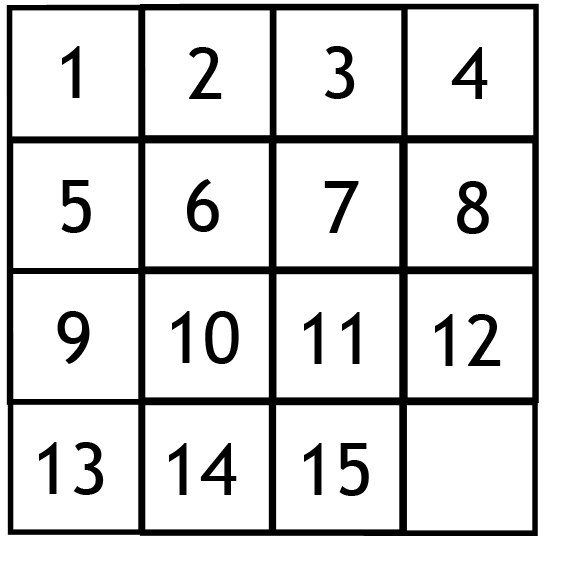
\includegraphics[scale=0.2]{input/pics/MagicPuzzle.png}}
	\hspace{0.02\textwidth}
	\subfloat[\myCaption{Figure of Magic Puzzle with inverse numbers.}]{\label{fig:MagicPuzzleInverse}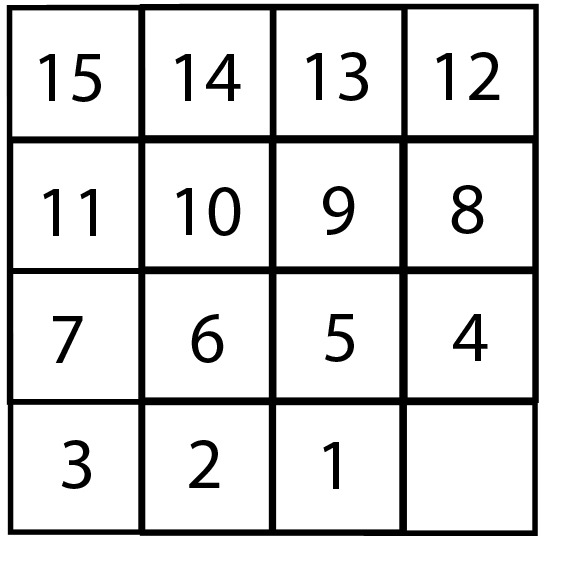
\includegraphics[scale=0.2]{input/pics/MagicPuzzle15-1}}
	\caption{\myCaption{Illustrations of the legal and illegal permutations of the Magic Puzzle.}}
	\label{fig:mpuzzles}
\end{figure}

\begin{comment}
	\begin{figure}[!h]
	\begin{center}
	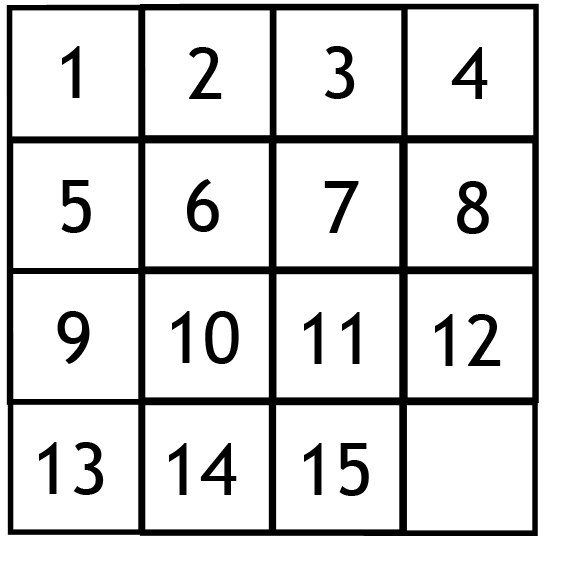
\includegraphics[scale=0.2]{input/pics/MagicPuzzle.png}
	\caption{\myCaption{Figure of Magic Puzzle.}}
	\label{fig:MagicPuzzle}
	\end{center}
	\end{figure}
	
	\begin{figure}[!h]
	\begin{center}
	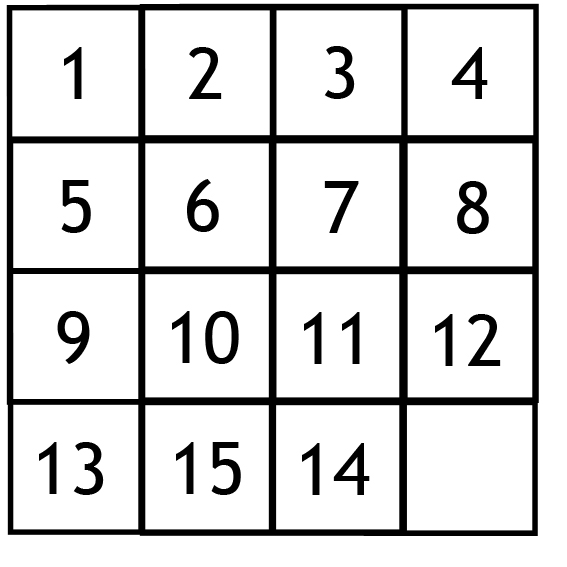
\includegraphics[scale=0.2]{input/pics/MagicPuzzle15-14.jpg}
	\caption{\myCaption{Figure of Magic Puzzle with inverse numbers.}}
	\label{fig:MagicPuzzleInverse}
	\end{center}
	\end{figure}
\end{comment}

For instance we got the figure \ref{fig:MagicPuzzle} and want to switch the tiles to be positioned like on figure \ref{fig:MagicPuzzleInverse} \cite[pp. 48-50]{Larsen81}. This permutation requires an odd transposition of the seven pairs (1,15), (2,14), (3,13), (4,12), (5,11), (6,10) and (7,9). This permutation is not possible because it requires an even number of transpositions to get the empty square at the same position. If we color the contraption like a chess board (see figure \ref{fig:Chess}) we can see that every odd transposition makes the empty square change color and with every even transposition the empty square lands on a square of the same color.

\textit{Did we put in the right picture in \ref{fig:MagicPuzzleInverse}?}

\begin{figure}[!h]
\begin{center}
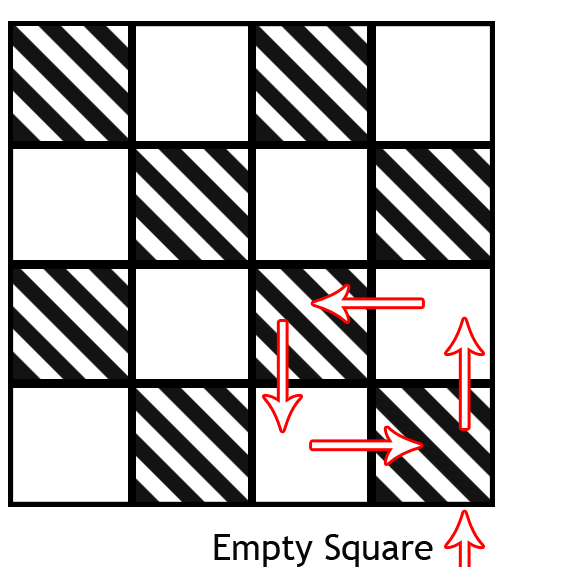
\includegraphics[scale=0.2]{input/pics/MagicPuzzle(EmptySquare).png}
\caption{\myCaption{Figure of Empty Square.}}
\label{fig:Chess}
\end{center}
\end{figure}

Therefore the number of different positions is $\frac{16!}{2}$. But if the empty square has to be in a fixed position then the possible permutations is $\frac{15!}{2}$. These permutations are almost like the ones the \rubik{} uses and they actually inspired \erno{} into his creation of the \rubik{} \cite[pp. 7-9]{Rubik87}. %input/introduction/recreationalMathematics/magicPuzzle %Denne sti skal bruges n�r rapporten samles!

